% This is text associated with the open textbook "Open Electromagnetics"
% See immediately below for author, date
% This work is licensed under the Creative Commons Attribution-ShareAlike 4.0 International License. (CC BY-SA 4.0) 
% To view a copy of the license, visit http://creativecommons.org/licenses/by-sa/4.0/

%ORB TITLE Gauss' Law for Magnetic Fields: Integral Form 
%ORB AUTHOR 0        # S.W. Ellingson, Virginia Tech (ellingson@vt.edu)
%ORB DATE 20180628   # yyyymmdd
%ORB ABSTRACT Gauss' Law for Magnetic Fields: Integral Form  

\label{m0018_Gauss_Law_Magnetic_Integral_Form} % <-- Must match name of this file and module directory name.  Don't mess with this!
\index{Gauss' law!magnetic field|(}

Gauss' Law for Magnetic Fields (GLM) is one of the four fundamental laws of classical electromagnetics, collectively known as \emph{Maxwell's Equations}.
Before diving in, the reader is strongly encouraged to review Section~\ref{m0003_Magnetic_Flux_Density}.
In that section, GLM emerges from the ``flux density'' interpretation of the magnetic field.  GLM is not identified in that section, but now we are ready for an explicit statement:
%
%ORB HIGHLIGHT
\begin{mdframed}[backgroundcolor=yellow!20,nobreak=true] 
\emph{Gauss' Law for Magnetic Fields} (Equation~\ref{m0018_eGLM}) states that the flux of the magnetic field through a closed surface is zero.
\end{mdframed}
%
This is expressed mathematically as follows:
%
\begin{equation}
\boxed{
\oint_{\mathcal S} {\bf B}\cdot d{\bf s} = 0
}
\label{m0018_eGLM}
\end{equation}
%
where 
${\bf B}$ is magnetic flux density and
${\mathcal S}$ is a closed surface with outward-pointing differential surface normal $d{\bf s}$.
It may be useful to consider the units.
${\bf B}$ has units of Wb/m$^{2}$; therefore, integrating ${\bf B}$ over a surface gives a quantity with units of Wb, which is magnetic flux, as indicated above.

GLM can also be interpreted in terms of magnetic field lines.  For the magnetic flux through a closed surface to be zero, every field line entering the volume enclosed by ${\mathcal S}$ must also exit this volume -- field lines may not begin or end within the volume.
The only way this can be true for every possible surface ${\mathcal S}$ is if magnetic field lines always form closed loops. 
This is in fact what we find in practice, as shown in Figure~\ref{m0018_fGLMBarMagnet}.
%
\begin{figure}
\begin{center}
\pdftooltip{{  % note double braces
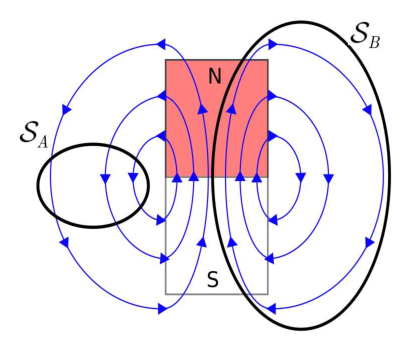
\includegraphics[width=\columnwidth]{modules/m0018_fGLMBarMagnet.eps}
% https://commons.wikimedia.org/wiki/File:M0018_fGLMBarMagnet_(2).svg
}}{A bar magnet oriented vertically with the north pole at the top. The magnetic field is shown by two sets of concentric curves labeled "B" that mirror each other on the left and right sides of the magnet. They are centered on the horizontal axis where the north and south poles meet. The left-side curves have arrows that indicate counterclockwise direction. The right-side curves have a clockwise direction. A large, bold oval lays over the middle of the curves on the left, labeled S sub A. A larger, bold oval lays over all of the curves on the right, labeled S sub B.}
\end{center} 
\centerline{\scriptsize 
\copyright~\hyperref[m0018_fGLMBarMagnet_Credit]{Youming / K.\ Kikkeri} 
\href{https://creativecommons.org/licenses/by-sa/4.0/}{CC BY~SA 4.0} 
} 
\caption{
\label{m0018_fGLMBarMagnet}
Gauss' Law for Magnetostatics applied to a two-dimensional bar magnet.  
For the surface ${\mathcal S}={\mathcal S}_A$, every field line entering ${\mathcal S}$ also leaves ${\mathcal S}$, so the flux through ${\mathcal S}$ is zero.
For the surface ${\mathcal S}={\mathcal S}_B$, every field line within ${\mathcal S}$ remains in ${\mathcal S}$, so the flux through ${\mathcal S}$ is again zero.
}
\end{figure}

Following this argument one step further, GLM implies there can be no particular particle or structure that can be the source of the magnetic field (because then that would be a start point for field lines).
This is one way in which the magnetic field is very different from the electrostatic field, for which every field line begins at a charged particle.
So, when we say that current (for example) is the source of the magnetic field, we mean only that the field coexists with current, and \emph{not} that the magnetic field is somehow attached to the current.
Summarizing, there is no ``localizable'' quantity, analogous to charge for electric fields, associated with magnetic fields.  This is just another way in which magnetic fields are weird! 

Summarizing:
%
%ORB HIGHLIGHT
\begin{mdframed}[backgroundcolor=yellow!20,nobreak=true] 
Gauss' Law for Magnetic Fields requires that magnetic field lines form closed loops.  Furthermore, there is no particle that can be identified as the source of the magnetic field.  
\end{mdframed}


{\bf Additional Reading:}
\begin{itemize}
\item ``\href{https://en.wikipedia.org/wiki/Gauss'_law_for_magnetism}{Gauss' Law for Magnetism}'' on Wikipedia.
\item ``\href{https://en.wikipedia.org/wiki/Maxwell's_equations}{Maxwell's Equations}'' on Wikipedia.
\end{itemize}

\index{Gauss' law!magnetic field|)}
